% !TeX encoding = UTF-8
% !TeX program = upLaTeX + dvipdfmx

\documentclass[dvipdfmx]{beamer}
\mode<presentation>
\usepackage{bxdpx-beamer}  % ナビゲーションシンボルを機能させる
\usepackage{pxjahyper}     % しおりの文字化け対策
\renewcommand{\kanjifamilydefault}{\gtdefault} % 和文既定をゴシックに変更

\usepackage{tikz}
\usetikzlibrary{positioning}

\usetheme{Frankfurt}

\setbeamertemplate{navigation symbols}{}   % ナビゲーションシンボルを消す
\setbeamertemplate{footline}[frame number] % フッターをスライド番号だけにする
\setbeamertemplate{blocks}[rounded][shadow=false]
\setbeamertemplate{caption}[numbered]

% \section ごとに目次を挿入
\AtBeginSection[]{%
  \begin{frame}
    \tableofcontents[currentsection]
  \end{frame}
}

\title{Learning Convolutional Neural Networks for Graphs}
\author{pione30}
\date{\today}

\begin{document}

  \frame[plain]{\titlepage}

  \frame[plain]{\Large All of the figures in this presentation are, unless explicitly stated, those of the original paper\footnote{http://proceedings.mlr.press/v48/niepert16.pdf}.}

\section*{Outline}

  \begin{frame}
    \tableofcontents
  \end{frame}

\section{Absract}

  \begin{frame}{Absract}

    \alert{We propose a framework for learning Convolutional Neural Networks (CNN) for arbitrary graphs.}
  \end{frame}

  \begin{frame}{Absract}

    \begin{block}{We claim that \dots }
      \begin{itemize}
        \item{the learned feature representations are competitive with state of the art graph kernels.} 
        \item{computation is highly efficient.}
      \end{itemize}
    \end{block}
  \end{frame}

\section{Introduction}

  \begin{frame}{The architecture of CNN}
    \begin{figure}[h]
      \centering
      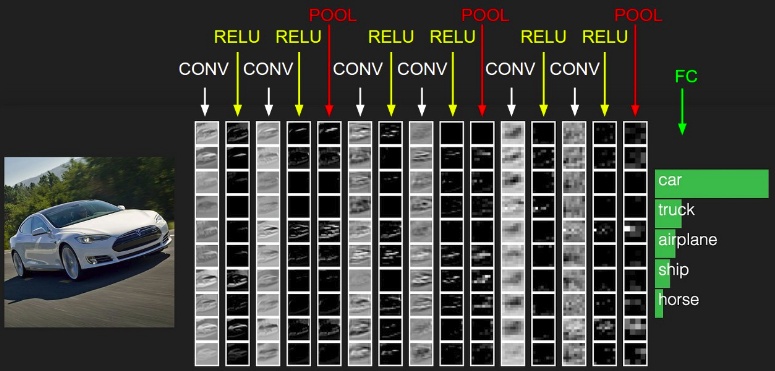
\includegraphics[width=0.8\paperwidth]{img/CS231n-CNN-architecture.png}
      \caption{The architecture of CNN\footnote{http://cs231n.github.io/convolutional-networks/}}
    \end{figure}
  \end{frame}

  \begin{frame}{The neighborhood graph of CNN}
    \begin{figure}[h]
      \centering
      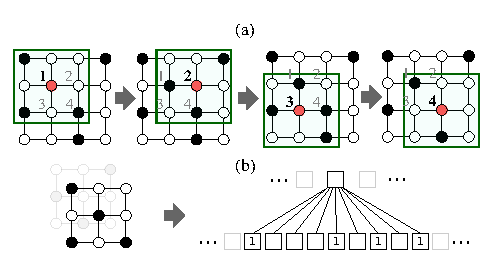
\includegraphics[width=0.8\paperwidth]{img/Fig1.pdf}
      \caption{A CNN with a receptive field of size 3x3.}
    \end{figure}
  \end{frame}

  \begin{frame}{The neighborhood graph of CNN}
    \begin{block}{CNN for images \dots}
      Due to \structure{the implicit spatial order} of the pixels, the sequence of nodes \
      for which neighborhood graphs are created is \alert{uniquely determined.}
    \end{block}
  \end{frame}

  \begin{frame}{Collection of \alert{arbitrary} graphs}
    \begin{block}{One has to \dots}
      \begin{enumerate}
        \item determin the node sequences for which neighborhood graphs are created
        \item compute a \alert{normalization} of neighborhood graphs, that is, \
          a unique mapping from a graph representation into a vector space representation.
      \end{enumerate}
    \end{block}

    \vspace{1cm}
    \visible<2->{$\to$ We proposed new approach termed \alert{PATCHY-SAN.}}
  \end{frame}

  \begin{frame}{The architecture of PATCHY-SAN}
    \begin{figure}[h]
      \centering
      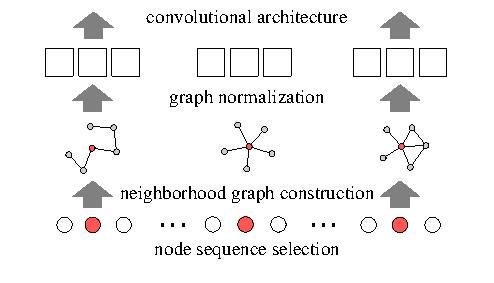
\includegraphics[width=0.8\paperwidth]{img/Fig2.pdf}
      \caption{An illustration of the PATCHY-SAN architecture.}
    \end{figure}
  \end{frame}

\section{Learning Procedure}

  \begin{frame}{Preparation}
    \begin{itemize}
      \item One has to determine a \alert{labeling procedure $\ell$} which is used to sort the graph and \
        select a node sequence.
      \item $\ell$ is also used when normalizing a neighborhood subgraph.
    \end{itemize}
  \end{frame}

  \begin{frame}{Architecture}
    \begin{figure}[h]
      \centering
      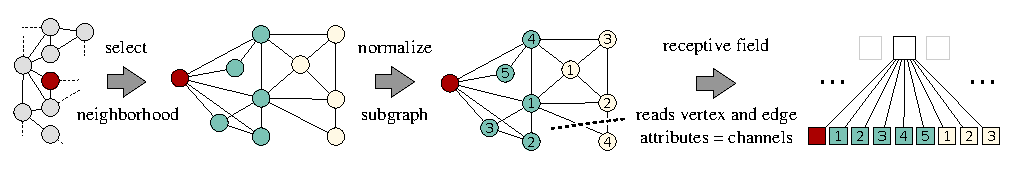
\includegraphics[width=0.9\paperwidth]{img/Fig3.pdf}
      \caption{The normalization procedure}
    \end{figure}
  \end{frame}

\section{Experiments}

  \begin{frame}{Runtime Analysis}
    PATCHY-SAN with 1-dimensional Weisfeiler-Lehman (1-WL) algorithm for the normalization.
    \vspace{5mm}

    \begin{block}{input graphs (graph-tool\footnotemark collection)}
      \begin{itemize}
        \item torus
        \item random
        \item power
        \item polbooks
        \item preferential
        \item astro-ph
        \item email-enron
      \end{itemize}
    \end{block}
    \footnotetext{https://graph-tool.skewed.de/}
  \end{frame}

  \begin{frame}{Runtime Analysis}
    \begin{figure}[h]
      \centering
      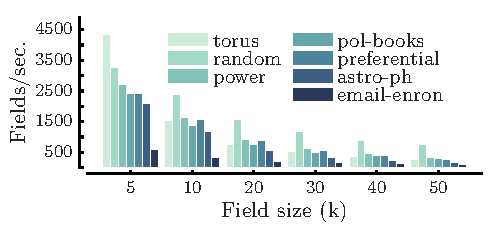
\includegraphics[width=0.8\paperwidth]{img/Fig4.pdf}
      \caption{Receptive fields per second rates on different graphs.}
    \end{figure} 
  \end{frame}

  \begin{frame}{Graph Classification}
    \begin{block}{Comparision: PATCHY-SAN with \dots}
      \begin{itemize}
        \item shortest-path kernel (SP)
        \item random walk kernel (RW)
        \item graphlet count kernel (GK)
        \item Weisfeiler-Lehman subtree kernel (WL)
      \end{itemize}
    \end{block}

    \begin{exampleblock}{Parameters}
      \begin{itemize}
        \item The decay factor for RW is chosen from $\{10^{-6}, 10^{-5}, \dots, 10^{-1}\}$
        \item The size of the graphlets for GK is 7
        \item THe height parameter of WL is 2
      \end{itemize}
    \end{exampleblock}
  \end{frame}

  \begin{frame}{Graph Classification}
    \begin{block}{Data sets}
      \begin{itemize}
        \item MUTAG
        \item PCT
        \item NCI1
        \item NCI109
        \item PROTEIN
        \item D\&D 
      \end{itemize}
    \end{block}
  \end{frame}

  \begin{frame}{Graph Classification}
    \begin{figure}[h]
      \centering
      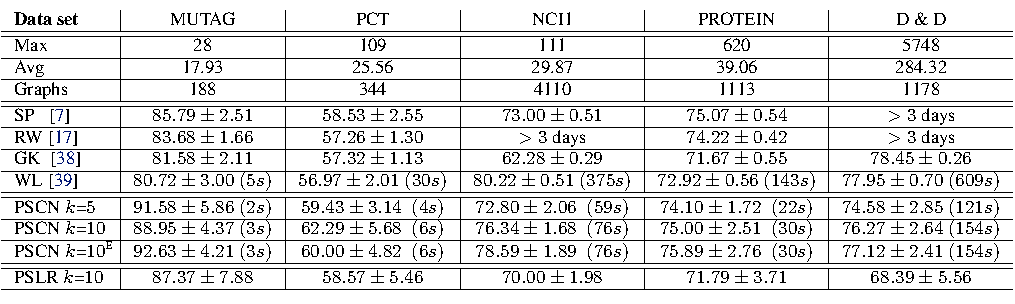
\includegraphics[width=0.8\paperwidth]{img/Table1.pdf}
      \caption{Properties of the data sets and accuracy and timing results (in seconds)}
    \end{figure} 
  \end{frame}

\section{Conclusion and Future Work}

  \begin{frame}{Conclusion}
    \alert{\Large We proposed a framework for learning graph representations that are especially beneficial in conjunction with CNNs.}
    \vspace{5mm}

    \begin{block}{Procedure}
      \begin{enumerate}
        \item select a sequence of nodes
        \item generate local normalized neighborhood representations for each of the nodes in the sequence
      \end{enumerate}
    \end{block}
  \end{frame}

  \begin{frame}{Future Work}
    \begin{itemize}
      \item RNNs
      \item different receptive field sizes
      \item pretraining with RBMs and autoencoders
      \item statistical relational models
    \end{itemize}
  \end{frame}

\end{document}
